To create the LSTM network, the \textit{Keras} framework within Python was used \citep{chollet2015keras}. There are several powerful tools for building machine learning models, but \textit{Keras} was chosen because of the ease of use and ability to take advantage of hyperparameter tuning when optimizing the model. The initial steps of model creation involved imputation (discussed in Section \ref{sec:EVER}), creating a simple model that could be made more complex over time, and splitting the data into a testing and training set. The testing set was chosen to be the first 90\% of the data between 1995 and 2023, leaving the remaining 10\% for testing. The initial model contained a single LSTM layer with 128 nodes, each of which used the ReLU activation function. Once the initial model was trained, code was adapted from \cite{lstmkeras} to get out-of-sample predictions. All code is available on \href{https://github.com/lliucci/Writing-Project}{GitHub}.

Once a base framework and method for validation was created, the structure of the model could be tweaked. This was done by implementing a random search across a set parameter space. The base model contained 3 LSTM layers and 3 Dropout layers. Parameters that were defined to be searched within each LSTM layer were the number of nodes (minimum of 8 with a maximum of 64) and the activation function (either ReLU or Tanh). For the Dropout layers, the dropout rate was chosen to be either 1\%, 5\%, 10\%, or 15\%. Fixed parameters include the kernel regularizer (L1 norm with a rate of 0.001) and the activity regularizer (L2 norm with a rate of 0.001).

The random search comprised of 50 randomly chosen combinations that were trained for 30 iterations each. The best model was chosen as the model with the lowest mean squared-error when compared to the testing data set. Once the best model was chosen, it was trained for an additional 20,500 iterations. A figure containing the training progress is shown in Figure \ref{fig:Training}. A key thing to note from the training process is that after about 12,000 iterations, the model performance becomes fairly constant with only minor improvements over time.

\begin{figure}[ht]
    \subfloat[2,530]{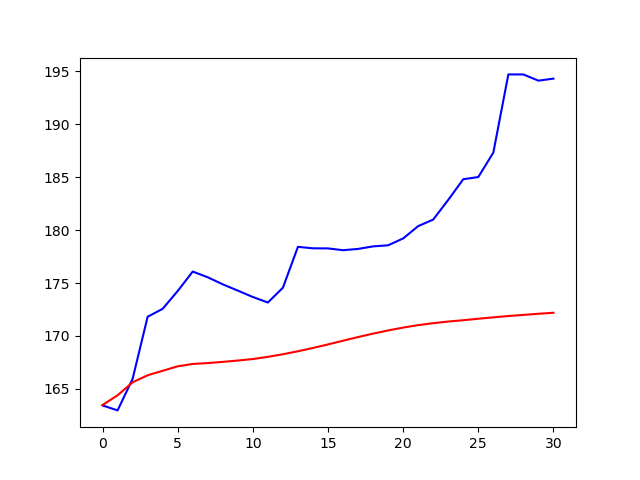
\includegraphics[width = 0.2\linewidth]{"../../Model Diagnostics/model_0.png"}}
    \subfloat[4,530]{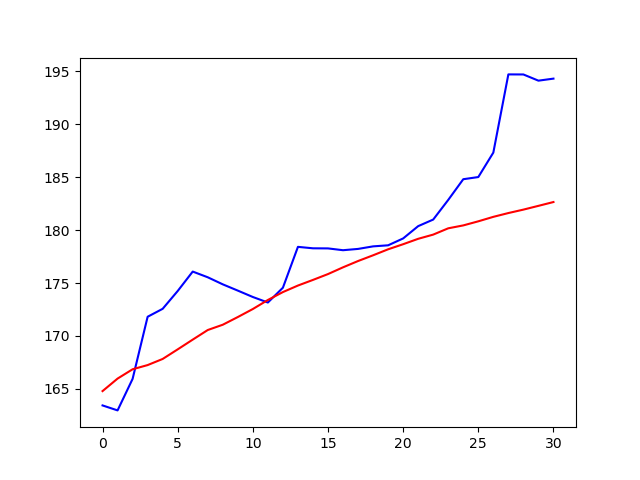
\includegraphics[width = 0.2\linewidth]{"../../Model Diagnostics/model_1.png"}}
    \subfloat[6,530]{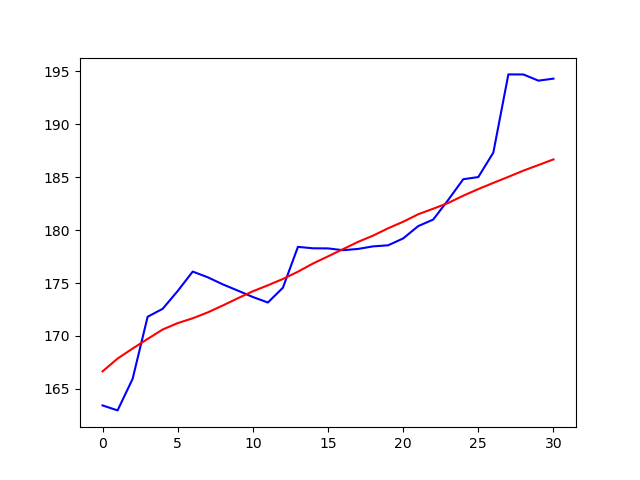
\includegraphics[width = 0.2\linewidth]{"../../Model Diagnostics/model_2.png"}}
    \subfloat[8,530]{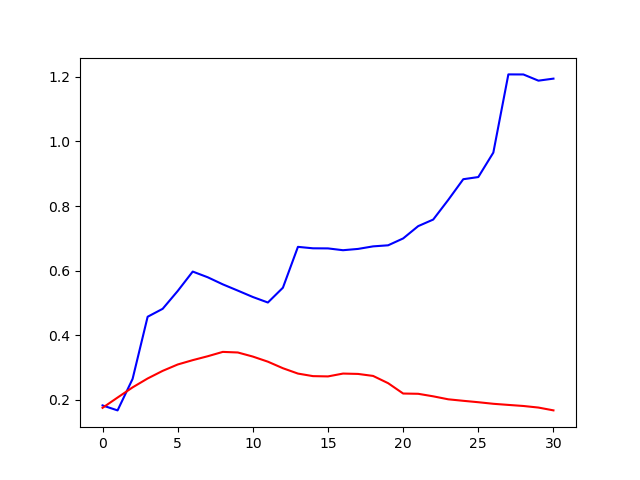
\includegraphics[width = 0.2\linewidth]{"../../Model Diagnostics/model_3.png"}}
    \subfloat[10,530]{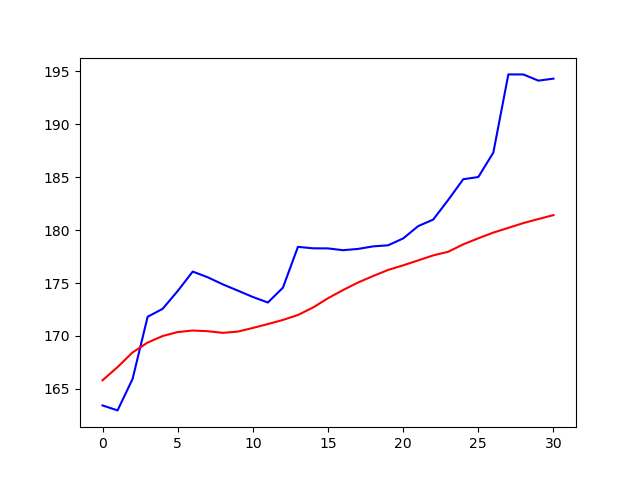
\includegraphics[width = 0.2\linewidth]{"../../Model Diagnostics/model_4.png"}}\\
    \subfloat[12,530]{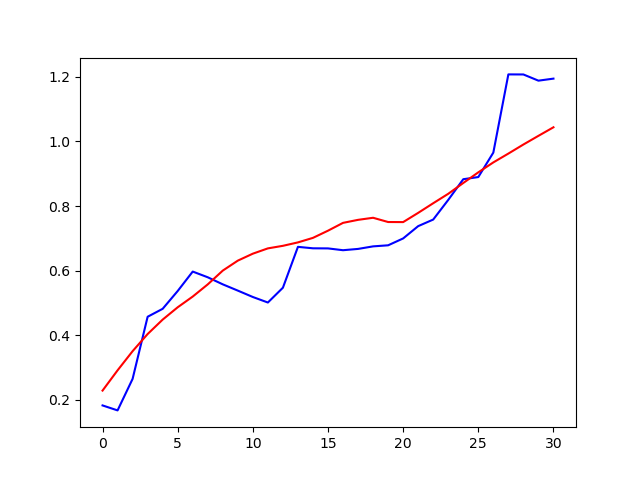
\includegraphics[width = 0.2\linewidth]{"../../Model Diagnostics/model_5.png"}}
    \subfloat[14,530]{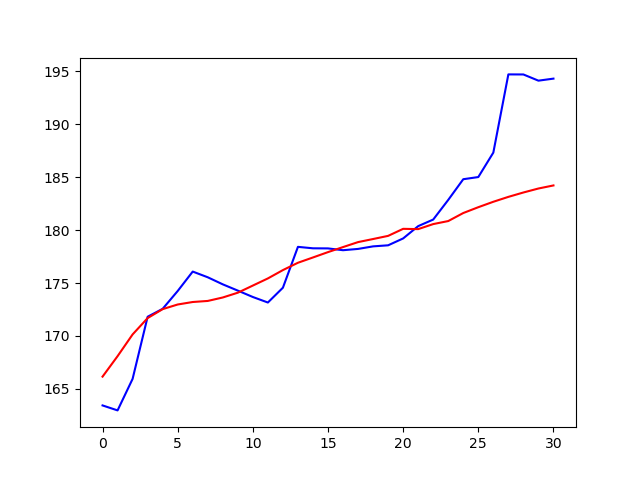
\includegraphics[width = 0.2\linewidth]{"../../Model Diagnostics/model_6.png"}}
    \subfloat[16,530]{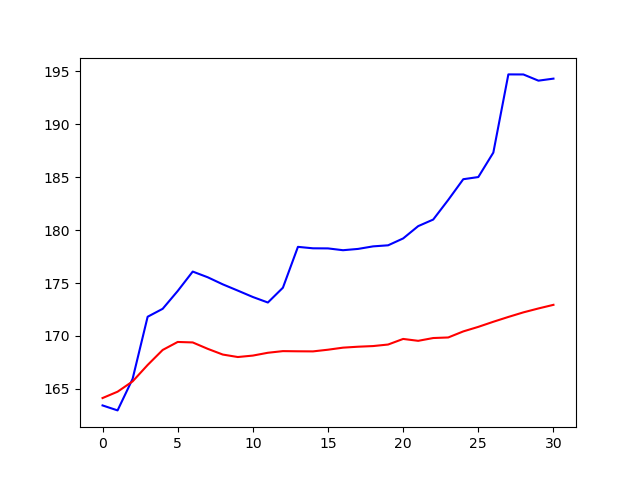
\includegraphics[width = 0.2\linewidth]{"../../Model Diagnostics/model_7.png"}}
    \subfloat[18,530]{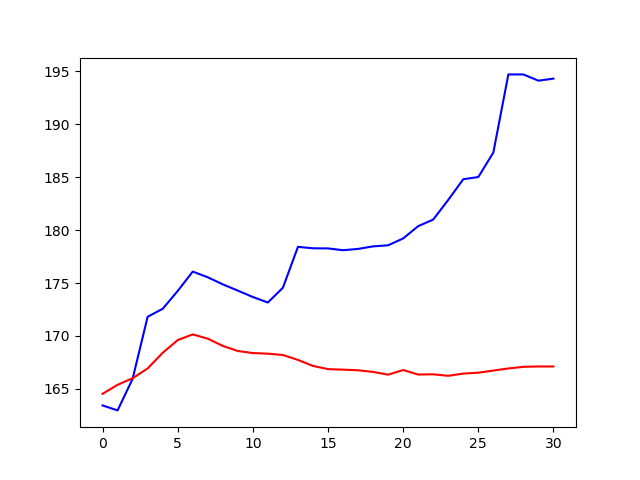
\includegraphics[width = 0.2\linewidth]{"../../Model Diagnostics/model_8.png"}}
    \subfloat[20,5530]{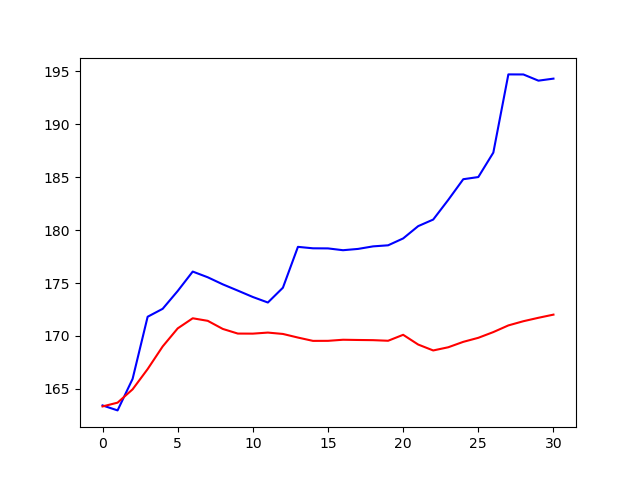
\includegraphics[width = 0.2\linewidth]{"../../Model Diagnostics/model_9.png"}}
    \caption{A series of plots obtained from the training process. Each plot shows the predicted water depths 31 days past the training set. The red line indicates the predictions from the LSTM and the blue line indicates the observed water depth. The number below each plot indicates how many generations the LSTM was trained for when the predictions were made.}
    \label{fig:Training}
\end{figure}